\modeCorrection

%%%% début de la page

\renewcommand{\thesubsection}{\textcolor{red}{\Roman{section}.\arabic{subsection}}}
\renewcommand{\thesubsubsection}{\textcolor{red}{\Roman{section}.\arabic{subsection}.\alph{subsubsection}}}

\setcounter{section}{0}
\setcounter{document}{0}
\sndEnTeteTPCinq

\begin{center}
\begin{mdframed}[style=titr, leftmargin=60pt, rightmargin=60pt, innertopmargin=7pt, innerbottommargin=7pt, innerrightmargin=8pt, innerleftmargin=8pt]

\begin{center}
\large{\textbf{TP 5 : Estimation de la concentration d'une solution colorée à l'aide d'une échelle de teintes
}}
\end{center}


\end{mdframed}
\end{center}

%%%% objectifs
\begin{tcolorbox}[colback=blue!5!white,colframe=blue!75!black,title=Objectifs de la séance :]
\begin{itemize}
    \item Réaliser une échelle de teintes
    \item Choisir et utiliser la verrerie adaptée pour préparer une solution par dilution,
    \item Encadrer la valeur d’une concentration en masse à l’aide d’une échelle de teinte.
\end{itemize}
\end{tcolorbox}

%%%% Consignes
\begin{tcolorbox}[colback=red!5!white,colframe=red!75!black,title= Consignes :]
\begin{itemize}
    \item Réaliser le travail en binôme,
    \item Faire attention à la verrerie lors de son utilisation,
    \item Respectez les consignes d'utilisation de la salle de chimie.
\end{itemize}
\end{tcolorbox}

%%%% contexte

\begin{tcolorbox}[colback=orange!5!white,colframe=orange!75!black,title= Scénario:]
\begin{wrapfigure}{r}{0.5\textwidth}
\vspace{-0.6cm}
    \centering
      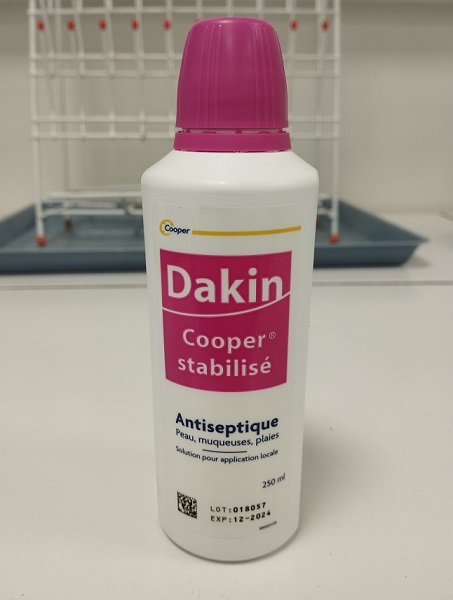
\includegraphics[width=0.4\textwidth]{Images/TP5/Dakin.jpg}
  \end{wrapfigure}
L’eau de Dakin est une solution aqueuse de couleur rose pâle et à l’odeur d’eau de Javel, elle est utilisée pour le lavage de la peau et des muqueuses.\\
C’est au cours de la première guerre mondiale que le chimiste américain Henri Dakin et le chirurgien français Alexis Carrel mettent au point cet antiseptique.\\
L’eau de Dakin est à base d’hypochlorite de sodium \chemform{NaClO}, qui en est le principe actif, et de permanganate de potassium \chemform{KMnO_4}, qui lui donne sa coloration rose et qui permet de stabiliser la solution vis-à-vis de la lumière.\\

\problematique{Afin de s'assurer de la qualité de ce flacon, on souhaite estimer la concentration en masse de permanganate de potassium dans un flacon d’eau de Dakin. Comment fait-on ?}
\end{tcolorbox}
\newpage

\begin{mdframed}[style=autreexo]
\textbf{\bsc{Liste du matériel}}
\begin{itemize}
    \item une solution aqueuse $S_0$ de permanganate de potassium \chemform{KMnO_4} de concentration en masse $C_{m,0}=80$~mg.L$^{-1}$, 
    \item une pissette d'eau distillée,
    \item des béchers,
    \item des pipettes jaaugées de 1mL, 2mL, 5mL, 10mL et 20mL,
    \item des fioles jaugées de 50mL,
    \item des pipettes Pasteur en plastique,
    \item des tubes à essais et leur support.    
\end{itemize}
\end{mdframed}


%%%% documents
\begin{doc}{La dilution}
Le principe est de prélever un certain volume d'une solution concentrée initiale appelée \textcolor{red}{solution mère} puis d'y ajouter de l'eau pour obtenir une solution moins concentrée appelée \textcolor{red}{solution fille} :
\begin{center}
    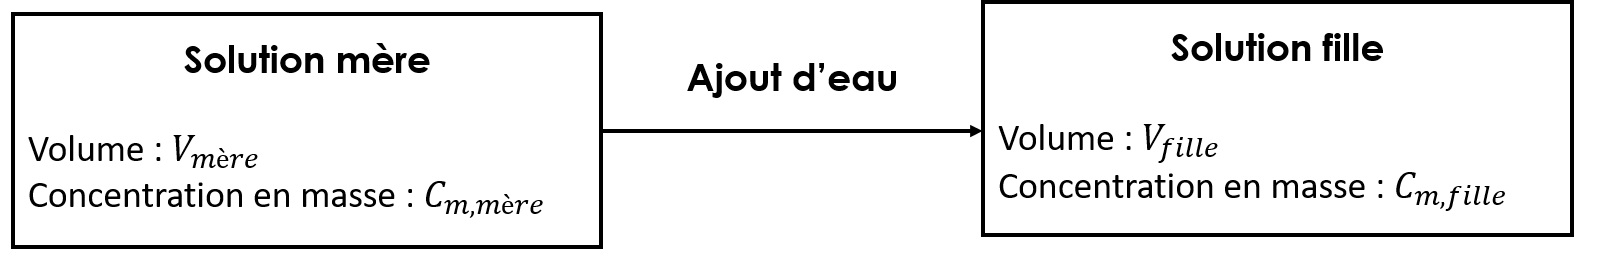
\includegraphics[scale=0.59]{Images/TP5/Dilution2.png}
\end{center}
\begin{tcolorbox}[colback=red!5!white,colframe=red!75!black,title=\textbf{Propriété de la dilution : }]
Au cours d'une dilution, la masse de soluté prélevée se conserve :
\begin{empheq}[box=\fbox]{align*}
    m_{\text{prélevée, mère}} &= m_{\text{soluté, fille}}\\
    C_{m,\text{mère}}V_{\text{prélevé}} &= C_{m,fille}V_{\text{fille}}
\end{empheq}
On peut dès lors définir le \textcolor{red}{facteur de dilution}, noté $F$ de la manière suivante :
\begin{equation*}
    F=\frac{C_{m,\text{mère}}}{C_{m,fille}} = \frac{V_{\text{fille}}}{V_{\text{prélevé}}}
\end{equation*}
\end{tcolorbox}
\end{doc}
\newpage
%%%%
\begin{doc}{Protocole expérimental de préparation d'une solution aqueuse par dilution}
\vspace{-0.8cm}
\begin{center}
    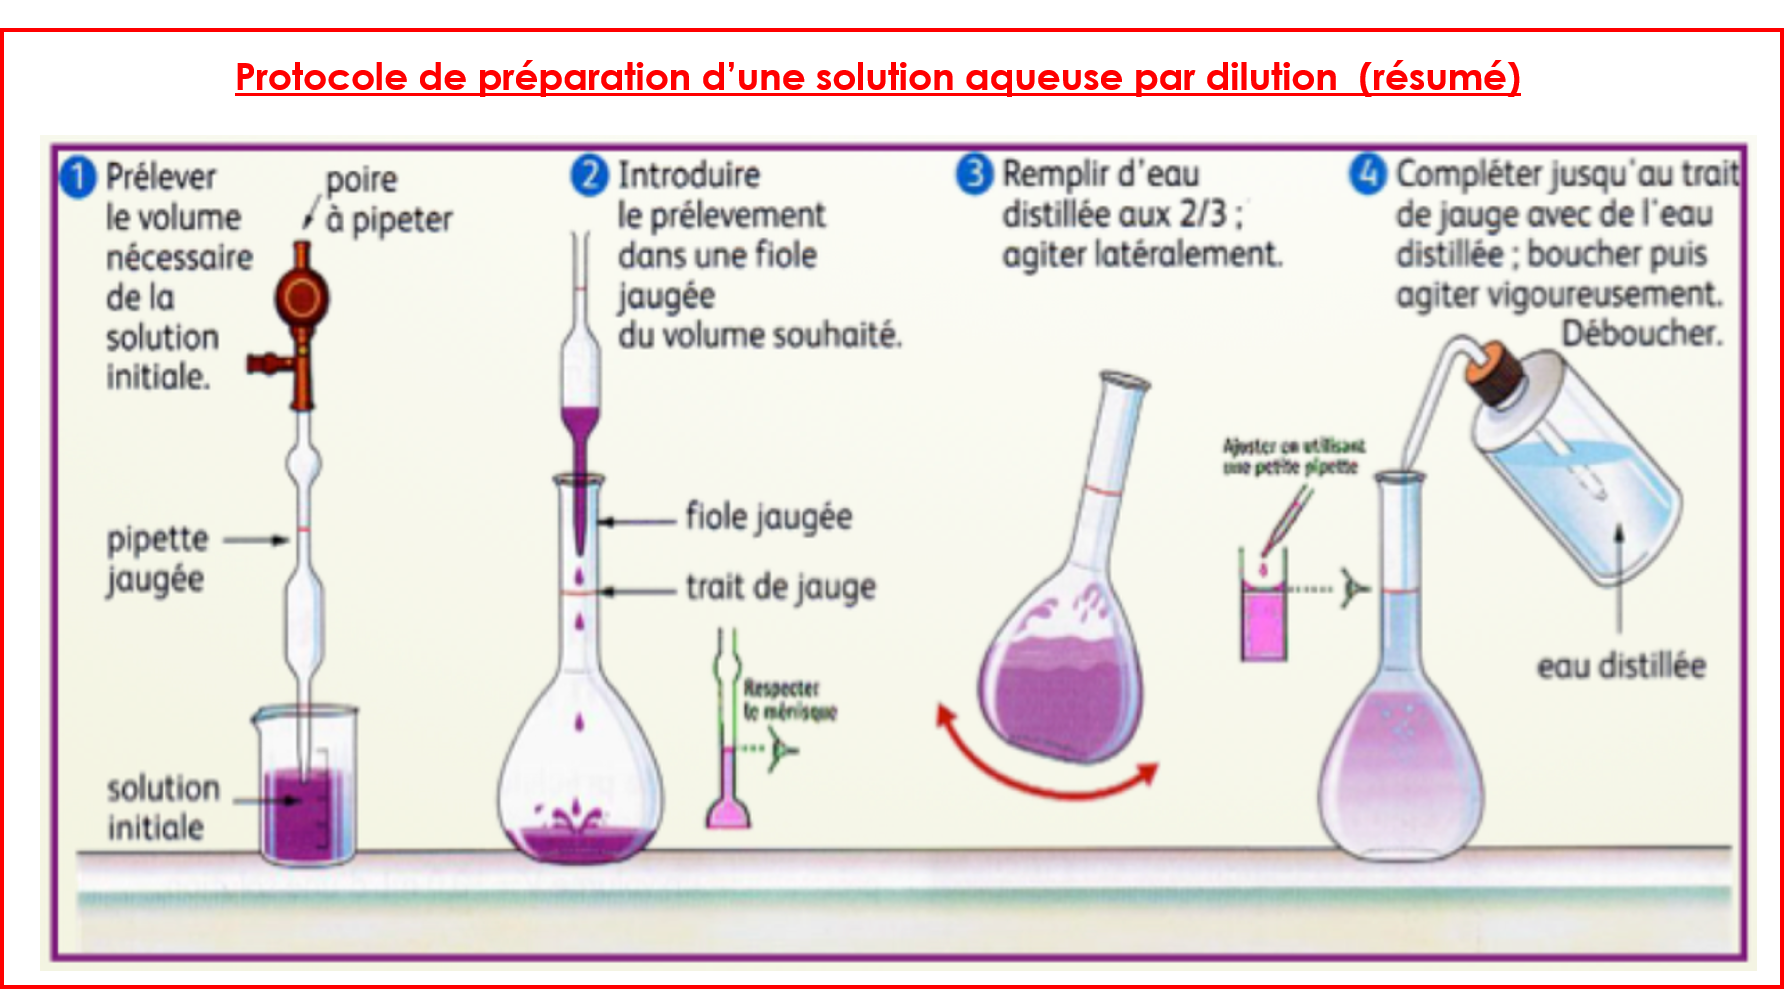
\includegraphics[scale=0.5]{Images/TP5/Protocole_dilution.png}
  \end{center}
  
  \begin{enumerate}
    \item Prélever un volume $V_\text{mère}$ de la solution mère à l'aide de la pipette jaugée.
    Le bas du ménisque doit atteindre la graduation supérieure.
    \item Introduire la solution prélevée dans la fiole jaugée de volume $V_\text{fille}$.
    \item Ajouter de l'eau distillée dans la fiole jaugée jusqu'aux $2/3$ et agiter doucement. 
    \item Ajouter goutte à goutte de l'eau distillée avec une pipette Pasteur jusqu'à ce que le bas du ménisque atteigne le trait de jauge (\textcolor{red}{vérifier à l'\oe il}),
    \item Fermer la fiole avec un bouchon et l'agiter en la retournant plusieurs fois.
    \item Verser la solution fille obtenue dans un bécher.
    \end{enumerate}
\end{doc}


%%%%
\newpage
\begin{doc}{\'{E}tiquette d'un flacon d'eau de Dakin commercial}
\vspace{-0.4cm}
  \label{doc:dakin}
  \begin{center}
      \begin{tabular}{|C{0.2}|C{0.25}|C{0.25}|c|}
      \hline
       & Soluté & Concentration en masse & Couleur\\
       \hline 
          Principe actif & Hypochlorite de sodium \chemform{NaClO} & 0,500~g de chlore actif pour 100~mL & Incolore (en solution)\\
          \hline
          \multirow{3}{*}{Principe non actifs} & Permanganate de potassium \chemform{KMnO_4} & 0,0010~g pour 100mL & Violet (en solution)\\
           & Dihydrogénophosphate de sodium déshydraté & Non connue (excipient) & Blanc (solide) \\
           & Eau purifiée & Non connue (excipient) & Incolore\\
           \hline
      \end{tabular}
  \end{center}
\end{doc}
 
%%%%

\begin{large}
    \textbf{\textcolor{red}{\underline{Travail à réaliser :}}}
\end{large}
\\
\question{Identifier le solvant de l'eau de Dakin et un soluté.}{L'eau de Dakin est une solution aqueuse. Par définition, l'eau est le solvant de cette solution.}{0}
\question{Parmis les solutés de l'eau de Dakin, identifier son principe actif et l'espèce chimique responsable de sa couleur.}{D'après le document 3, le principe actif est l'ion hypochlorite de sodium \chemform{NaClO} et l'espèce responsable de la couleur est le permanganate de potassium \chemform{KMnO_4}}{0}
\\
\question{Compléter le document 1 sur la propriété de la dilution.}{Voir le document 1.}{0}
\\
\question{On souhaite préparer quatre solutions, notées S$_{1}$, S$_{2}$, S$_{3}$ et S$_{4}$ à partir de la solution aqueuse S$_{0}$ de permanganate de potassium de concentration en masse $C_{m,0}=80$~mg.L$^{-1}$. Compléter le tableau ci-dessous \textbf{\underline{après avoir détaillé le calcul pour la solution S$_{1}$}} :
\begin{center}
    \begin{tabular}{|c|c|c|c|c|}
        \hline
        Solution fille & V$_{\text{mère à prélever}}$ (en mL) & V$_{\text{fille}}$ (en mL) & $C_{m,fille}$ (en mg.L$^{-1}$) & Facteur de dilution $F$\\
        \hline
         S$_{1}$ & 1  & 50,0  & 1,6 & 50 \\
         \hline
         S$_{2}$ & 2 & 50,0  & 3,2 & 25 \\
         \hline
         S$_{3}$ & 5 & 50,0  & 8,0 & 10 \\
         \hline
         S$_{4}$ & 10  & 50,0  & 16 & 5 \\
         \hline
         \textit{(Bonus)} S$_{5}$ & 15 & 50,0 & 24 & environ 3 \\
         \hline
         \textit{(Bonus)} S$_{6}$ & 20 & 50,0 & 32 & 2,5\\
         \hline
    \end{tabular}
\end{center}
}{}{0}\\
\question{En suivant le protocole du document 2 (et les explications du professeur), préparer les solutions S$_{1}$, S$_{2}$, S$_{3}$ et S$_{4}$.}{Fait en TP.}{0}
\\
\question{\`{A} votre avis, comment feriez-vous pour déterminer la concentration de la solution mère commerciale ?}{Il y a deux possibilités : 
\begin{itemize}
    \item Comme on sait que la solution est colorée et que la couleur provient des ions permanganates, on peut réaliser une échelle de teinte avec différentes concentrations en masse $C_m$ d'ions permanganates et comparer la teinte à celle de la solution commerciale (c'est ce qu'on va faire ici),
    \item mesurer la masse volumique de chaque solution fille et réaliser une courbe d'étalonnage (c'est ce qu'on fera au TP 6).
\end{itemize}}{0}

\question{Remplir sur quelques centimètres les tubes à essais avec vos solutions filles. Attention à se rappeler la correspondance entre la solution dans le tube à essai et la solution $S$ correspondante.}{Effectué en TP.}{0}
\\
\question{Puis, déterminer \textbf{\underline{un encadrement}} de la concentration en masse en permanganate de potassium de la solution d'eau de Dakin commerciale.}{On trouve à l'aide de l'échelle de teintes réalisées : $8~\text{mg.L}^{-1}<C_{m,Dakin} < 16~\text{mg.L}^{-1}$}{0}
\\
\question{\`{A} partir des données de l'étiquette de la solution commerciale, calculer la concentration en masse de permanganate de potassium normalement présente dans la solution commerciale.}{Les données de l'étiquette donnent une concentration en masse égale à $C_{m,Dakin}=\frac{0,0010~\text{g}}{100~\text{mL}}=\frac{1,0~\text{mg}}{0,1~\text{L}}=10~\text{mg.L}^{-1}$}{0}
\\
\question{Vos résultats expérimentaux sont-ils en accord avec cette concentration en masse ? }{Oui, l'encadrement donne une concentration en masse de permanganate dans la solution de Dakin entre 8 et 16~mg.L$^{-1}$. Cet encadrement contient bien la valeur de $C_{m,Dakin}=10~\text{mg.L}^{-1}$.}{0}

\begin{center}
    
\includegraphics[scale=0.9]{Images/Feuilles/Grands_carreaux.pdf}
\end{center}
